\documentclass[11pt]{article}
\usepackage[margin=1in]{geometry}
\usepackage{amsmath, amssymb}
\usepackage{booktabs}
\usepackage{graphicx}
\usepackage{float}
\usepackage{caption}
\usepackage{subcaption}
\usepackage{siunitx}
\sisetup{round-mode=places,round-precision=3}

\title{Econ 8210 --- Problem Set \#1 \\ \large}
\author{Tate Mason}
\date{\today}

\newcommand{\figph}[1]{%
  \begin{center}
    \fbox{\rule{0pt}{90pt}\rule{0.95\linewidth}{0pt}}\\
    \vspace{0.3em}\small\textit{#1 (insert figure here)}
  \end{center}
}

\newcommand{\matfive}{%
\left[
\begin{array}{ccccc}
\cdot & \cdot & \cdot & \cdot & \cdot \\
\cdot & \cdot & \cdot & \cdot & \cdot \\
\cdot & \cdot & \cdot & \cdot & \cdot \\
\cdot & \cdot & \cdot & \cdot & \cdot \\
\cdot & \cdot & \cdot & \cdot & \cdot \\
\end{array}
\right]
}

\begin{document}
\maketitle

\tableofcontents
\bigskip

\section{Data Import and Descriptive Statistics}

\subsection{Descriptive Table of Market Statistics}
\begin{table}[H]
\centering
\caption{Market-Level Descriptive Statistics}
\begin{tabular}{lcccc}
\toprule
\textbf{Variable} & \textbf{Mean} & \textbf{SD} & \textbf{Median} & \textbf{Max} \\
\midrule
\# Brands per market & 34.9 & 4.82 & 37 & 39 \\
\# Manufacturers per market & 3.95 & 0.259 & 4 & 4 \\
Total sales per market & 15,555 & 12,358 & 12,557 & 84,657 \\
Brand-level sales per market & 446 & 726 & 238 & 26470 \\
Price & 0.235 & 0.0265 & 0.233 & 0.325 \\
Fiber (g/serving) & 1.3 & 0.0874 & 1.31 & 1.67 \\
Sugars (g/serving) & 8.31 & 0.205 & 8.33 & 10.2 \\
\bottomrule
\end{tabular}
\end{table}

\subsection{Time Series: Average Price and Sales}
\begin{figure}[H]
\centering
  
\includegraphics[width=0.8\textwidth]{q12-ts-1.pdf}
\caption{Average Price of Cereal Over Time}
\end{figure}

\begin{figure}[H]
\centering
  
\includegraphics[width=0.8\textwidth]{q12-ts-2.pdf}
\caption{Average Sales of Cereal Over Time}
\end{figure}

\begin{figure}[H]
\centering
  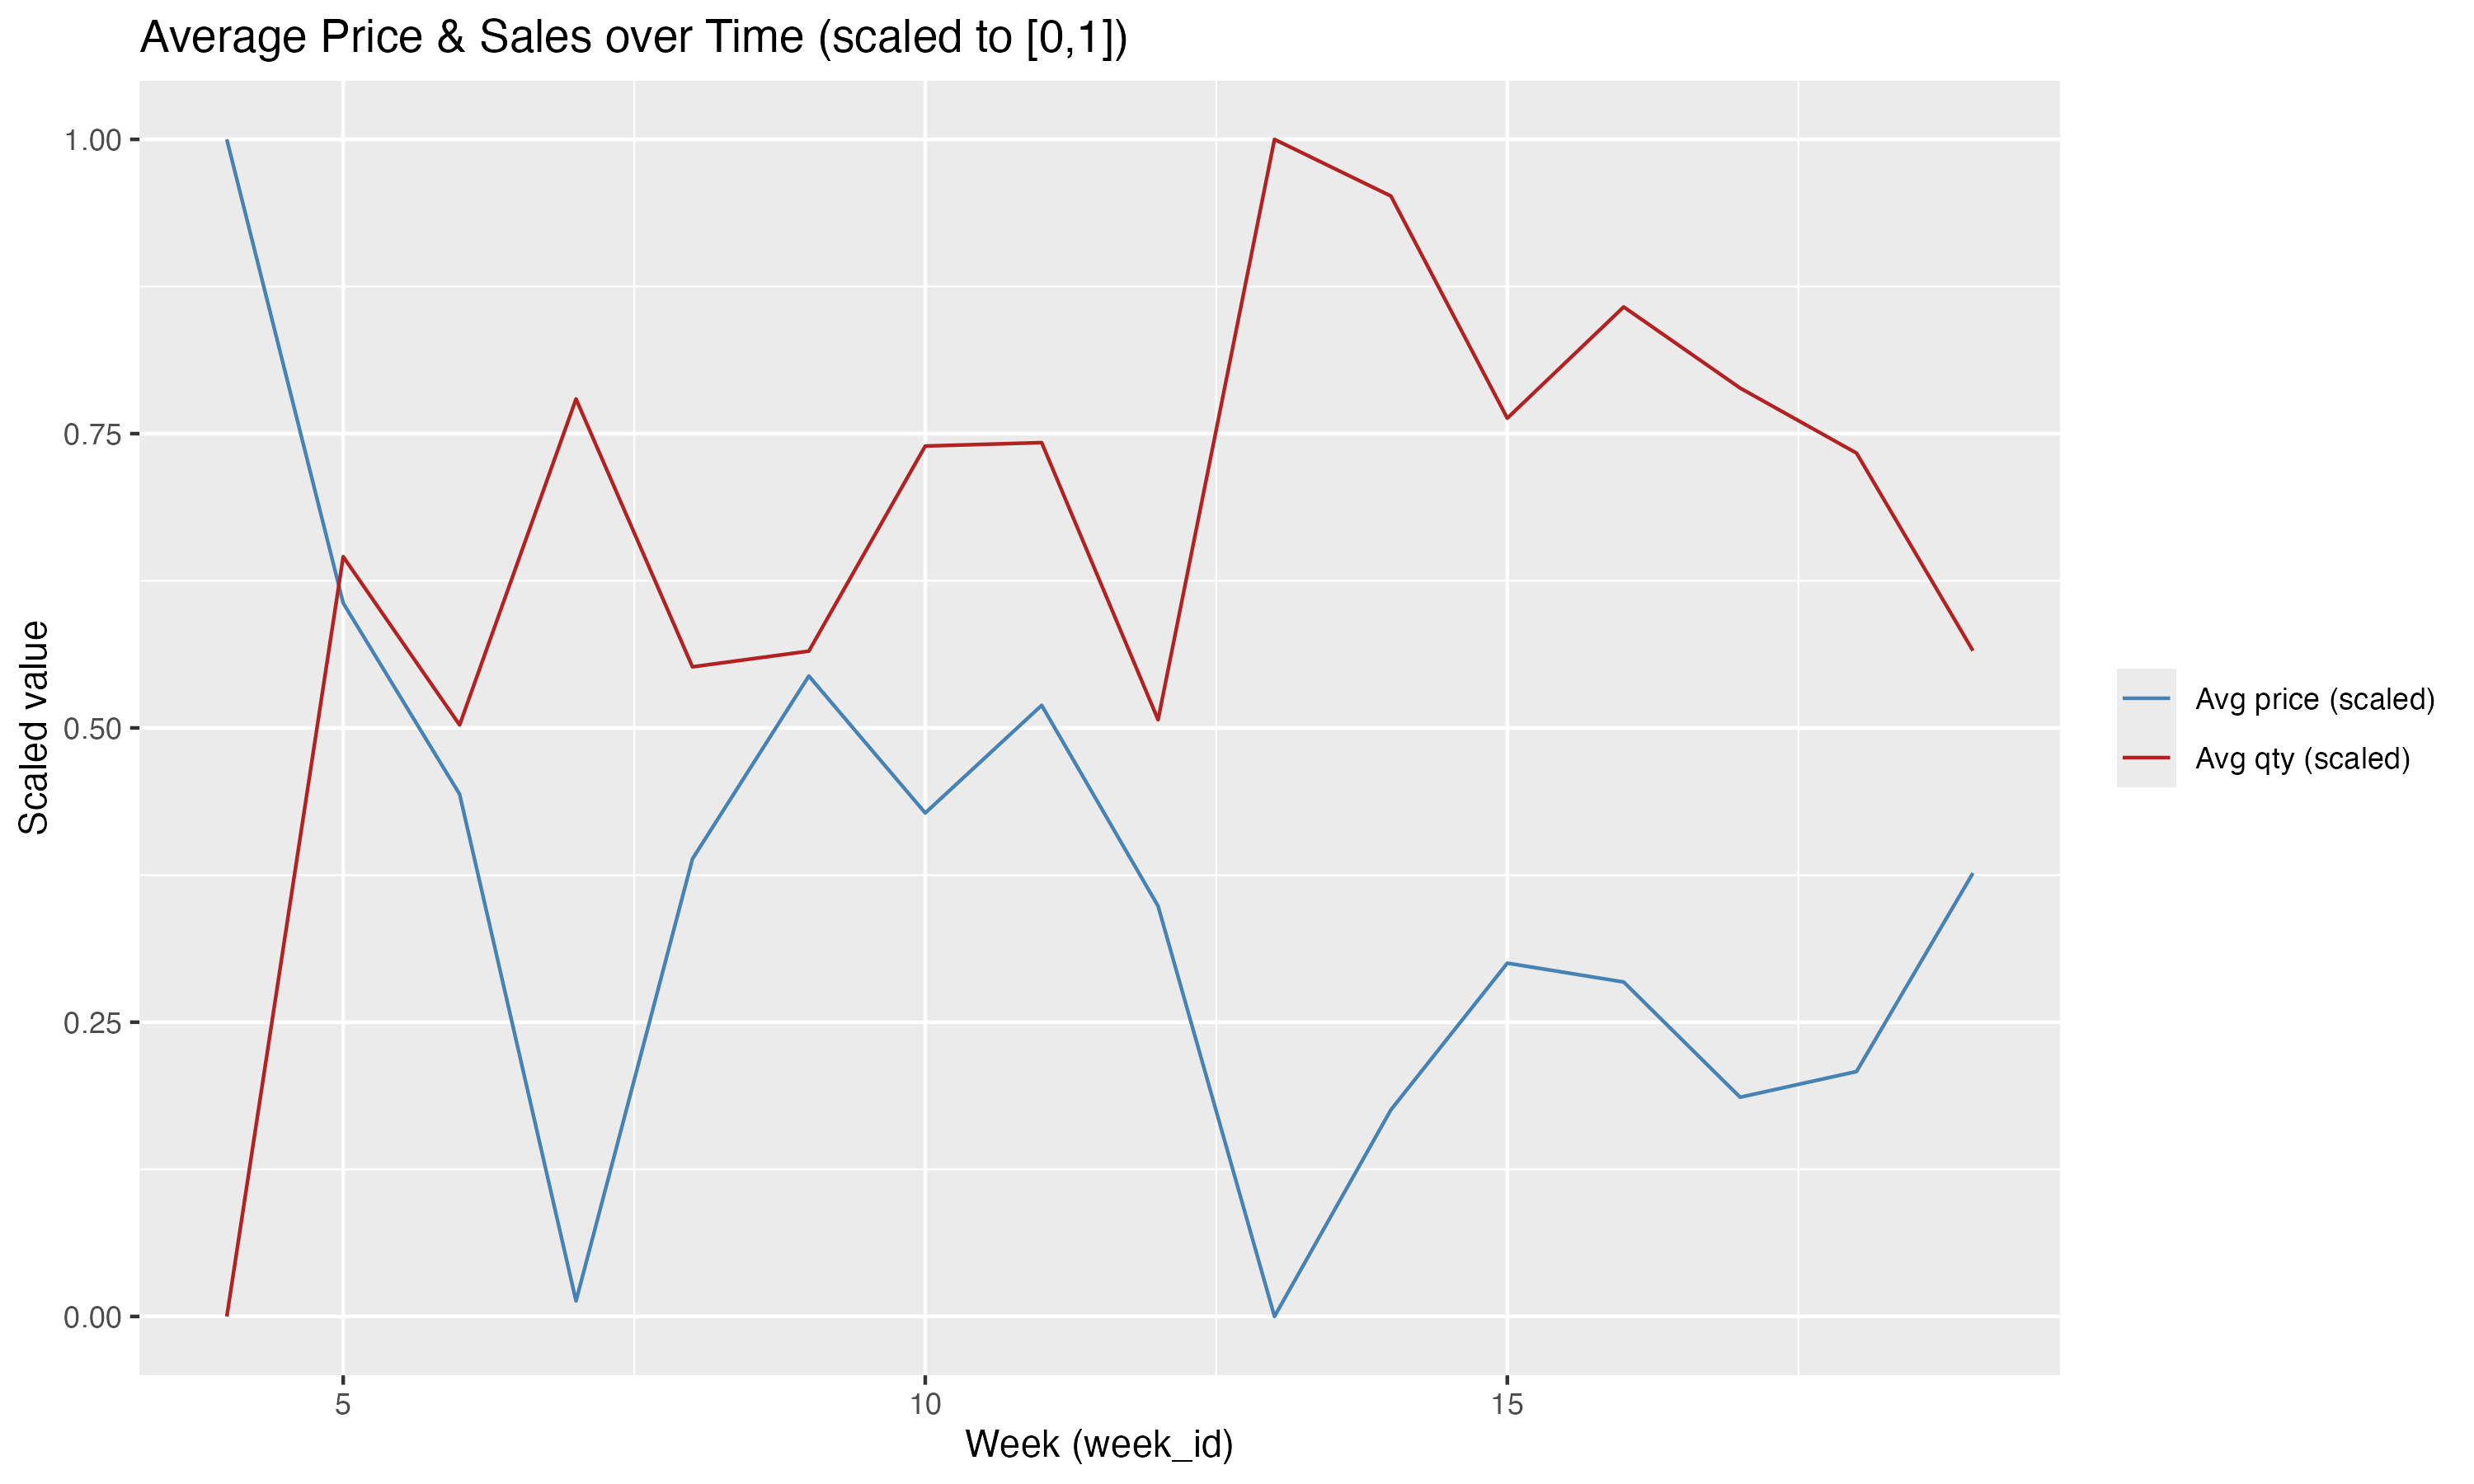
\includegraphics[width=0.8\textwidth]{q12-ts-3.png}
\caption{Average Price and Sales of Cereal Over Time}
\end{figure}

Interestingly, price and sales cross quite early in the time series. This is 
due to the negative relationship between price and sales. As price goes up, sales go down,
and vice versa. Thus, when price is high, sales are low, and when price is low, sales are high.

\subsection{HHI Over Time}
\begin{figure}[H]
\centering
  
\includegraphics[width=0.8\textwidth]{q13-hhi-1.pdf}
\caption{Average HHI (Brand) Over Time}
\end{figure}

\begin{figure}[H]
\centering
  
\includegraphics[width=0.8\textwidth]{q13-hhi-2.pdf}
\caption{Average HHI (Manufacturer) Over Time}
\end{figure}

\begin{figure}[H]
\centering
  
\includegraphics[width=0.8\textwidth]{q13-hhi-3.pdf}
\caption{Average HHI (Brand and Manufacturer) Over Time}
\end{figure}

The market has a fairly high level of concentration, with the average HHI being around 0.2 for brands and around 0.5 for manufacturers.

\section{Multinomial Logit and Nested Logit}

\subsection{Estimating Equation (MNL)}

\begin{equation}
  u_{jmt} = \alpha\cdot p_{jmt} + \beta\cdot \mathit{X}_{jmt} + \xi_{jmt} 
\end{equation}

\subsection{OLS Estimates (MNL)}
\begin{table}[H]
\centering
\caption{MNL OLS Estimates}
\begin{tabular}{l S[table-format=1.3] S[table-format=1.3]}
\toprule
 & {\textbf{Coef.}} & {\textbf{SE}} \\
\midrule
Price & -8.31 & 0.084 \\
Fiber & -0.12 & 0.003 \\
Sugars & -0.043 & 0.001 \\
Flavored (dummy) & 0.193 & 0.008 \\
Fortified (dummy) & 0.004 & 0.009 \\
\bottomrule
\end{tabular}
\end{table}

\begin{figure}[H]
\centering
  
\includegraphics[width=0.8\textwidth]{q2-2-1.pdf}
\caption{Histogram: Own-Price Elasticities (MNL, OLS)}
\end{figure}

\subsection{2SLS Estimates (MNL)}
\begin{table}[H]
\centering
\caption{MNL 2SLS Estimates}
\begin{tabular}{l S[table-format=1.3] S[table-format=1.3]}
\toprule
 & {\textbf{Coef.}} & {\textbf{SE}} \\
\midrule
Price & -62.764 & 7.898 \\
Fiber & -0.571 & 0.066 \\
Sugars & -0.121 & 0.012 \\
Flavored (dummy) & 0.179 & 0.023 \\
Fortified (dummy) & 0.377 & 0.060 \\
\bottomrule
\end{tabular}
\end{table}

\begin{figure}[H]
\centering
  
\includegraphics[width=0.8\textwidth]{q2-3-1.pdf}
\caption{Histogram: Own-Price Elasticities (MNL, 2SLS)}
\end{figure}

\subsection{Elasticity Matrix (Top 5 Brands, MNL)}
\paragraph{Average elasticity matrix across markets (own and cross):}
\[

\begin{table}[H]
\centering
\small
\setlength{\tabcolsep}{6pt}
\renewcommand{\arraystretch}{1.1}
\begin{tabular}{lrrrrr}
\toprule
 & \textbf{Kellogg Mini-Wheats} & \textbf{GM Cheerios} & \textbf{GM Honey Nut} & \textbf{Post HBO} & \textbf{Kellogg Flakes} \\
\midrule
\textbf{Kellogg Mini-Wheats} & -13.142 & 0.262 & 0.265 & 0.266 & 0.258 \\
\textbf{GM Cheerios}         & 0.264   & -13.267 & 0.267 & 0.268 & 0.260 \\
\textbf{GM Honey Nut}        & 0.265   & 0.264   & -13.231 & 0.269 & 0.258 \\
\textbf{Post HBO}            & 0.262   & 0.264   & 0.266   & -13.216 & 0.260 \\
\textbf{Kellogg Flakes}      & 0.267   & 0.263   & 0.265   & 0.269   & -13.285 \\
\bottomrule
\end{tabular}
\caption{Own (diagonal) and cross (off-diagonal) price elasticities}
\end{table}
\]
These mostly make sense, with own price changes causing massive changes in quantity demanded, with substitution to other brands.

\subsection{Manufacturer Markups (MNL Assumption: Independent Pricing)}
\begin{figure}[H]
\centering
  
\includegraphics[width=0.8\textwidth]{q2-5-1.pdf}
\caption{Average Manufacturer Markups (MNL; Independent Pricing)}
\end{figure}

\begin{table}[H]
  \centering
  \caption{Average Manufacturer Markups (MNL; Independent Pricing)}
  \begin{tabular}{l S[table-format=1.3]}
    \toprule
    \textbf{Brand} & \textbf{Avg. Markup} & \textbf{S.D. Markup}\\
    \midrule
    Ralcorp Holdings & 0.081 & 0.0225 \\
    Pepsico Inc. & 0.081 & 0.0179 \\
    Kelloggs & 0.076 & 0.0182 \\
    General Mills & 0.0634 & 0.0127 \\
  \bottomrule
  \end{tabular}
\end{table}

\subsection{Nested Logit: Data and Estimation}
\paragraph{Estimating equation (include $\sigma$):} 
\begin{equation}
  u_{jmt} = \alpha\cdot p_{jmt} + \beta\cdot \mathit{X}_{jmt} + \sigma_g\cdot s_{j|g} + \xi_{jmt}

\begin{table}[H]
\centering
\caption{Nested Logit 2SLS Estimates}
\begin{tabular}{l S[table-format=1.3] S[table-format=1.3]}
\toprule
 & {\textbf{Coef.}} & {\textbf{SE}} \\
\midrule
Price & -54.397 & 6.652 \\
Fiber & -0.487 & 0.0593 \\
Sugars & -0.101 & 0.0123 \\
Flavored  & 0.174 & 0.0202 \\
Forified & 0.300 & 0.0554 \\
$\sigma$ & 0.130 & 0.0790  \\
\bottomrule
\end{tabular}
\end{table}

\begin{figure}[H]
\centering
  
\includegraphics[width=0.8\textwidth]{q2-7-1.pdf}
\end{figure}

\subsection{Elasticity Matrix (Top 5 Brands, Nested Logit)}
\[

\begin{table}[H]
\centering
\small
\setlength{\tabcolsep}{6pt}
\renewcommand{\arraystretch}{1.1}
\begin{tabular}{lrrrrr}
\toprule
 & \textbf{Mini-Wheats} & \textbf{Cheerios} & \textbf{Honey Nut} & \textbf{Honey Bunches} & \textbf{Flakes} \\
\midrule
\textbf{Mini-Wheats} & -16.726 & 3.935 & 3.885 & 4.220 & 3.413 \\
\textbf{Cheerios}    & 3.804  & -16.887 & 4.515 & 4.865 & 4.028 \\
\textbf{Honey Nut}   & 3.770  & 4.376  & -16.826 & 4.791 & 3.976 \\
\textbf{Honey Bunches} & 4.272 & 5.006 & 4.941 & -16.782 & 4.387 \\
\textbf{Flakes}      & 3.286  & 3.795  & 3.808 & 4.280 & -16.887 \\
\bottomrule
\end{tabular}
\caption{Own- and cross-price elasticities for top cereal brands}
\end{table}
\]
\noindent\textit{Row/column order: top 5 brands by sales.}

These are similar to the MNL elasticities, but the own and cross elasticities are much larger in magnitude.
Cross elasticities are way too big, suggesting I had a coding error. I will diagnose and try to fix this.

\subsection{Manufacturer Markups (Nested Logit; Multi-Product Ownership)}
\begin{figure}[H]
\centering
  
\includegraphics[width=0.8\textwidth]{q2-9-1.pdf}
\caption{Average Manufacturer Markups (Nested Logit; Multi-Product Ownership)}
\end{figure}

\begin{table}[H]
\centering
\small
\setlength{\tabcolsep}{6pt}
\renewcommand{\arraystretch}{1.1}
\begin{tabular}{lrrrr}
\toprule
\textbf{Parent Firm} & \textbf{Avg. Markup} & \textbf{SD} & \textbf{Median} & \textbf{Max} \\
\midrule
Ralcorp Holdings & 0.0930 & 0.0259 & 0.0881 & 0.370 \\
PepsiCo Inc.     & 0.0929 & 0.0206 & 0.0907 & 0.261 \\
Kellogg’s        & 0.0873 & 0.0210 & 0.0839 & 0.210 \\
General Mills    & 0.0731 & 0.0146 & 0.0723 & 0.311 \\
\bottomrule
\end{tabular}
\caption{Summary of firm-level markups (nested logit model)}
\end{table}

\subsection{Diversion Ratios}
\paragraph{Average diversion ratios across markets:}
\begin{itemize}
  \item Cheerios $\rightarrow$ Corn Flakes: \dotfill
  \item Cheerios $\rightarrow$ Fruit Loops: \dotfill
\end{itemize}

\begin{table}[H]
\centering
\small
\setlength{\tabcolsep}{6pt}
\renewcommand{\arraystretch}{1.1}
\begin{tabular}{lrrr}
\toprule
 & \textbf{GM Cheerios} & \textbf{Kellogg Corn Flakes} & \textbf{Kellogg Froot Loops} \\
\midrule
\textbf{GM Cheerios}           & --     & 0.2322 & 0.0814 \\
\textbf{Kellogg Corn Flakes}   & 0.1009 & --     & 0.0814 \\
\textbf{Kellogg Froot Loops}   & 0.0814 & 0.0814 & --     \\
\bottomrule
\end{tabular}
\caption{Diversion Ratios}
\end{table}

These results seem to make sense, with corn flakes and cheerios being good substitues, and froot loops
being a weaker substitute for both. Froot Loops is a children's cereal, while the other two are more general audience cereals,
implying this makes sense.

\subsection{Merger Simulation Sketch}

\begin{table}[H]
\centering
\small
\setlength{\tabcolsep}{6pt}
\renewcommand{\arraystretch}{1.1}
\begin{tabular}{lr}
\toprule
\textbf{Merged Parent} & \textbf{Average Markup} \\
\midrule
Ralcorp Holdings & 0.0930 \\
PepsiCo Inc.     & 0.0929 \\
General Mills / Kellogg (GM\_K) & 0.0799 \\
\bottomrule
\end{tabular}
\caption{Average markups after firm mergers}
\end{table}

If General Mills and Kellogg were to merge, the new firm would have an average markup of 0.0799, which is lower than either firm's previous average markup.
This is because the merged firm would internalize the competition between its two brands, leading to lower markups. However, overall
market competition would decrease, potentially leading to higher prices for consumers, and increased market power.

\section{Mixed Logit}

\subsection{Specification and Instruments}
State the mixed logit specification, instruments, and random coefficients here.

\subsection{Estimates (Mixed Logit)}
\begin{table}[H]
\centering
\caption{Mixed Logit Estimates (Nonlinear + Linear Terms)}
\begin{tabular}{l S[table-format=1.3] S[table-format=1.3]}
\toprule
 & {\textbf{Coef.}} & {\textbf{SE}} \\
\midrule
$\alpha$ (price) & -5.42 & 9.054 \\
$\beta_{\text{fiber}}$ (level) & 0.251 & 0.443 \\
$\beta_{\text{sugars}}$ (level) & 0.241 & 0.4323 \\
$\beta_{\text{fiber}\times \text{inc}}$ & -0.160 & 2.834 \\
$\beta_{\text{sugars}\times \text{inc}}$ & -0.197 & 0.4435 \\
$\beta_{\text{sugars}\times \text{nchild}}$ & -128.959 & 1.655  \\
$\beta_{\text{fiber}\times \text{nchild}}$ & -24.982 & 0.5477  \\
$\sigma_{\text{fiber}}$ & 4.358e-07 & 0.6722 \\
$\sigma_{\text{sugars}}$ & 1.711e-07 & 2.2938 \\
\bottomrule
\end{tabular}
\end{table}

\begin{figure}[H]
\centering
  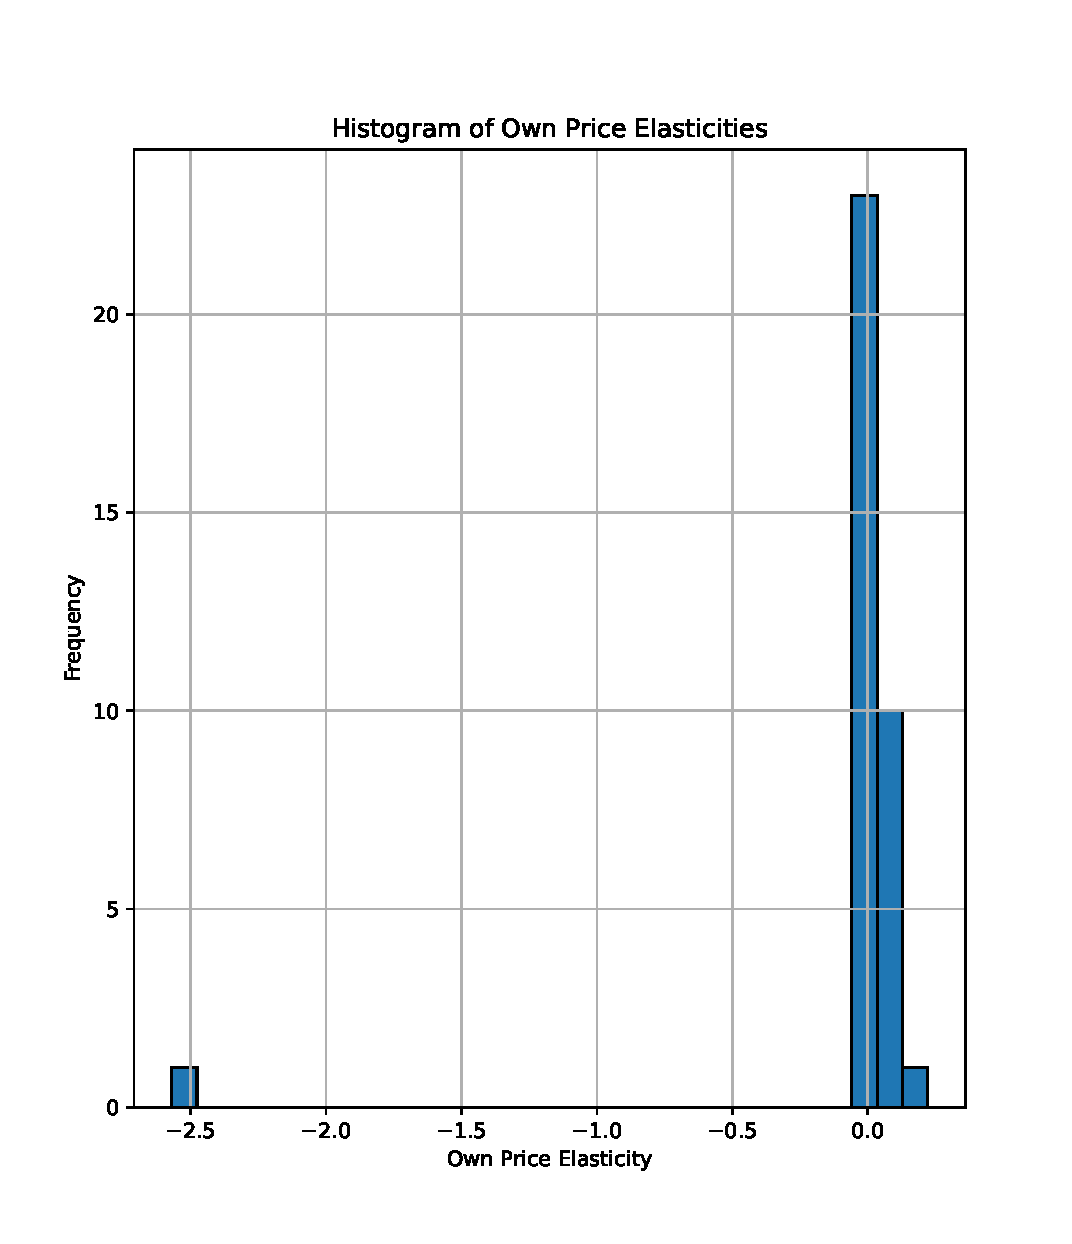
\includegraphics[width=0.8\textwidth]{3.1_hist.pdf}
\caption{Histogram: Own-Price Elasticities (Mixed Logit)}
\end{figure}

I was unable to get past this point due to time constraints. I am sorry, but I hope to finish this problem set soon. I will submit an updated version when I do.
I tried to get the mixed logit more correct, but unfortunately, I am clearly missing something important. I will continue to work on this. The estimates are all 
pretty wild, with most being insignificant and some having the wrong sign. I am not sure what is going wrong, but I will keep trying to fix it. However, it does
seem the instrument is fairly weak, and thus we are not able to get precise estimates.

\end{document}
